\chapter{Definitions}
This work proposes the application of a high availability technique to a context broker system. For a better understanding of the system and its development, definitions of Context, Context-Aware System, Context Representation, Fault Tolerance and High Availability related terms are presented.

\section{Context}
Context has had many definitions throughout the years. The first time Context was defined regarding the human-computer interaction was by \cite{schilit1994disseminating}, where context is defined related to location, identities of nearby people and objects, and the changes happening to those.  Similarly, \cite{brown1997context} define context as location, people around the user, time of day, season, temperature, etc. Many authors have also defined context using synonyms, as \cite{brown1995stick} had the idea of “environment”, i.e., what the computer knows about the user's environment, or \cite{franklin1998all} that see context as user's situation. Thus, a lot of definitions have existed, but they all end up being too specific. Context is about the whole situation of an application and its users, and we can't really.

\cite{dey2000providing} defined context as follows: ''Context is any information that can be used to characterize the situation of an entity. An entity is a person, place, or object that is considered relevant to the interaction between a user and an application, including the user and application themselves.'' This is the definition this work uses.

\subsection{Context-Aware System}
Like context, context-awareness has had several definitions over the years. The first definition was done by \cite{schilit1994disseminating}, and it restricted to applications informed about context and applications that adapt themselves to context. Later on, synonyms have been used to define a context-aware system: reactive \cite{cooperstock1995evolution}, responsive \cite{elrod1993responsive}, situated \cite{hull1997towards}, context-sensitive  \cite{rekimoto1998augment} and environment-directed \cite{fickas1997software}. All these definitions refer to either using context, adapting to context, or both.

The definition used in this work is provided by \cite{dey2000providing}: ''A system is context-aware if it uses context to provide relevant information and/or services to the user, where relevancy depends on the user's task.''

\subsection{How to represent Context}
According to \cite{dey2000providing}, context-aware applications deal with the who's, where's, when's and what's (the activities that are occurring) of entities, and interpret this information to define why a situation is occurring. The designer of the application must decide what to do with the information. Once we have the information available, either through automated sensors or through user's interference, we need to represent it in a way a machine can process and store it.

\cite{baldauf2007survey} presents and defines the most relevant context modeling options: key-value, markup scheme, graphical, object oriented, logic based and ontology based models. As this work is developed over the same base as \cite{crippa2010}, it uses the same context representation model: a markup scheme variation, ContextML \cite{knappmeyer2010contextml}. It is chosen as it provides **ver artigo do marcos pq escolheu cxml


\subsection{ContextML}

ContextML is an XML-based representation schema for context information, where it is categorized into scopes and related to different types of entities. It is designed to be used with REST-based communication between the framework components \cite{knappmeyer2010contextml}. 

The system consists on three core components: Context Provider, Context Consumer and Context Broker. They are briefly described below, based on definitions made by \cite{knappmeyer2010contextml}. 



\subsubsection{Context Representation}



\subsubsection{Context Provider}
A Context Provider (CxP) provides context information of a certain type, e.g. weather, location, activity, etc. It gathers data from sensors, network, user interactions, or other sources. A CxP is specialized in a specific domain of context information (location, weather etc).


\subsubsection{Context Consumer}
A Context Consumer (CxC) queries for and uses context data, e.g. is a context-aware application. A CxC can retrieve context information asynchronously through a subscription method, or by a synchronous method where it requests the Broker for a specific information or for a particular Provider interface, to query the Provider directly.

\subsubsection{Context Broker}
A Context Broker (CxB) is the central component of the architecture, and is the focus of this work. It handles and aggregates context information, and is an interface between the other architecture components. The CxB allows CxCs to subscribe to context information, and CxPs to provide this information. It also provides a lookup service, where the CxCs can query the CxB for CxPs that have a particular capability, depending on the CxC’s interest.

\subsubsection{Entity and Scope}
An entity is the subject of interest which context data refers to, and it is composed of two parts: a type and an identifier. The type refers to the category of the entity: username for human users, imei for mobile devices, room for a room with sensors, etc. The identifier specifies a particular item within a set of entities of the same type.

A scope is a set of closely related context parameters. Every context parameter has a name and belongs to only one scope. The parameters of a scope can only be requested, updated, provided and store at the same time, making the data always consistent. For example, a scope ‘position’ has latitude, longitude and accuracy attributes; any operation on this scope is performed on all these attributes: if the latitude is updated, so is the longitude and accuracy, what is correct, because otherwise it would not make sense. Entity-scope association is illustrated in Figure \ref{fig:entityscope}. \par

\begin{figure}[H]
	\centering
	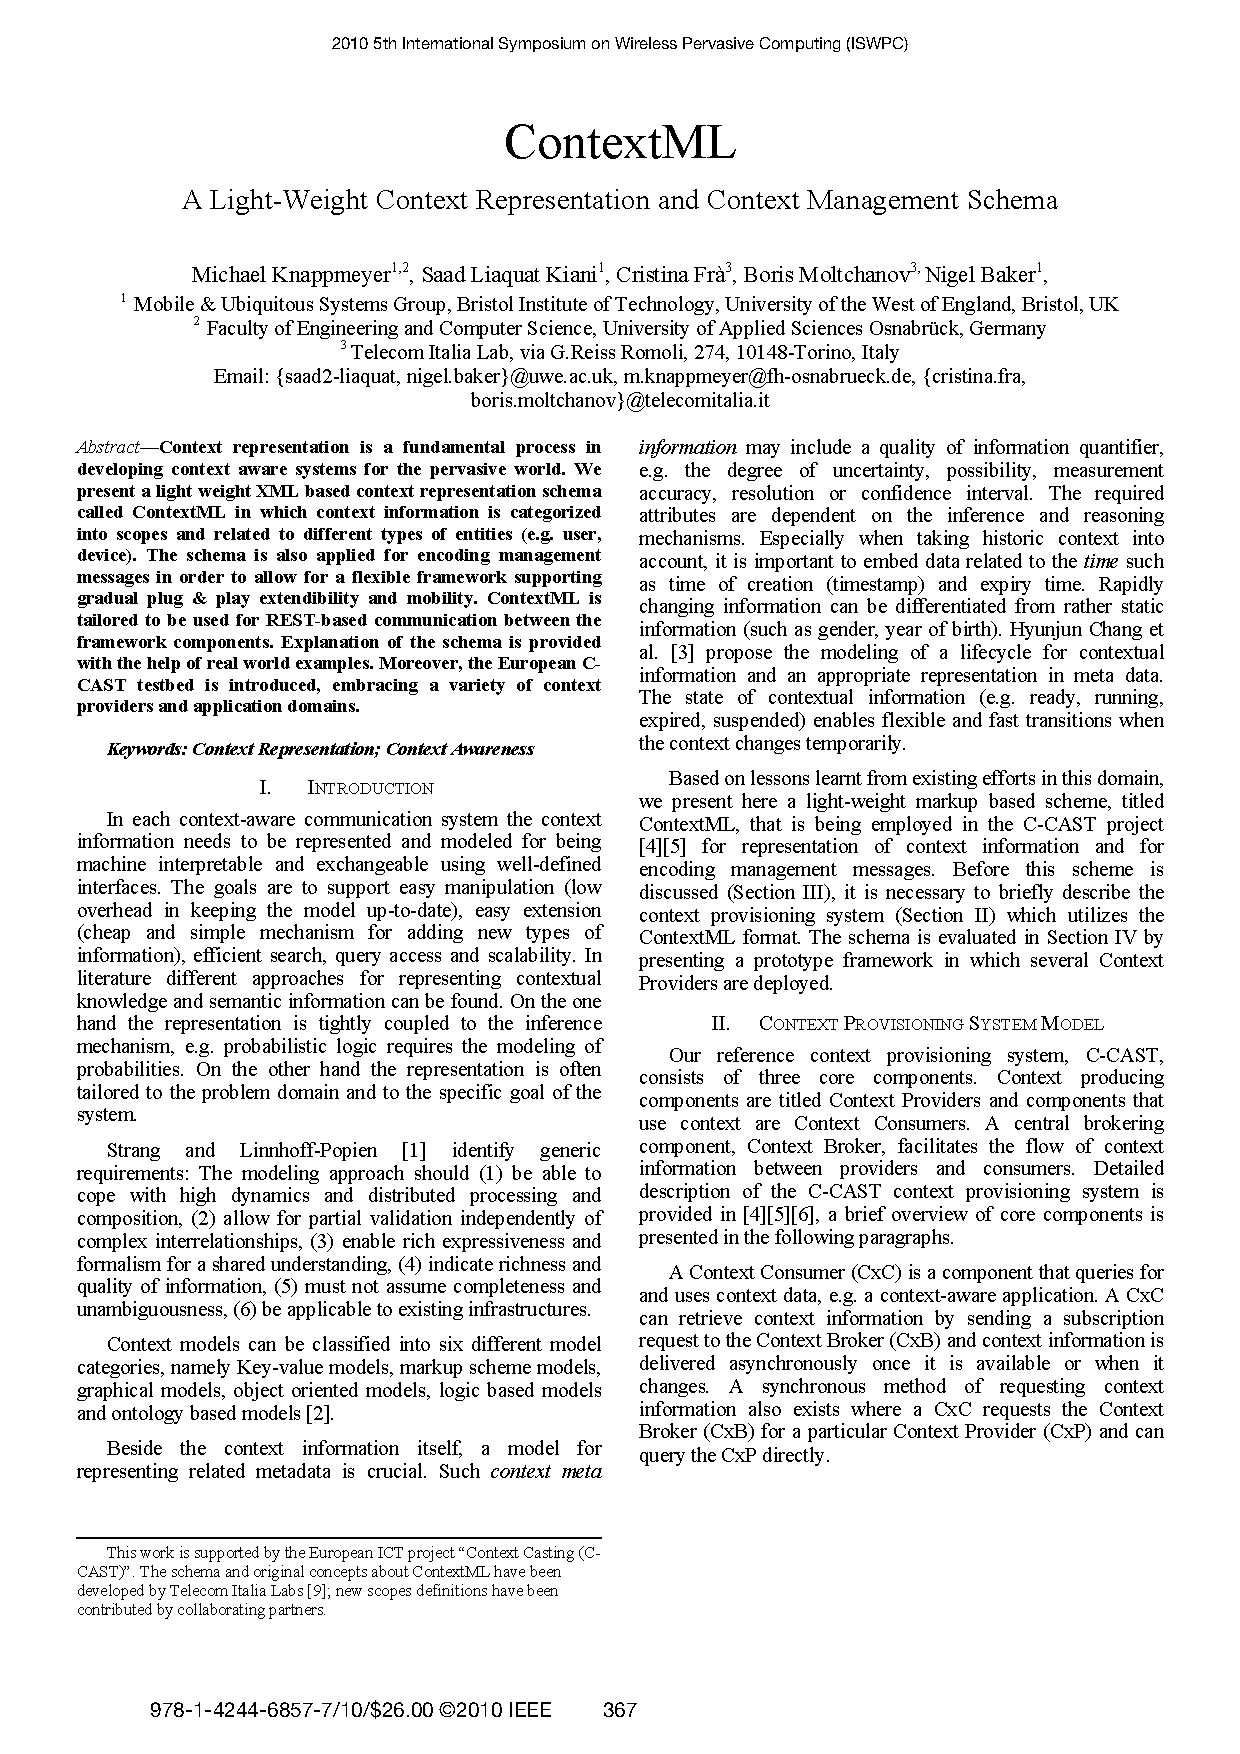
\includegraphics[scale=1]{entityscope.pdf}
	\caption{Entity and Scope relationship. Source: \cite{knappmeyer2010contextml}}
	\label{fig:entityscope}
	
\end{figure}

\subsubsection{Context Messages}


\section{Fault Tolerance}
\subsection{Dependable System}
\subsection{High Availability}
\subsubsection{Uses in real world}
\subsubsection{Problems involving High Availability}

